\documentclass{standalone}

\setlength{\unitlength}{1mm}
\usepackage{tikz}
\usetikzlibrary{calc}
\usetikzlibrary{shapes.geometric}

\usepackage{pgfplots}
\usepackage{fontawesome}
\usepackage{latexsym}

\pgfdeclarelayer{background}
\pgfdeclarelayer{foreground}
\pgfsetlayers{background,main,foreground}

\begin{document}
\pagestyle{empty}

\definecolor{orange}{RGB}{255,140,0}
\definecolor{DarkGreen}{RGB}{50,200,50}


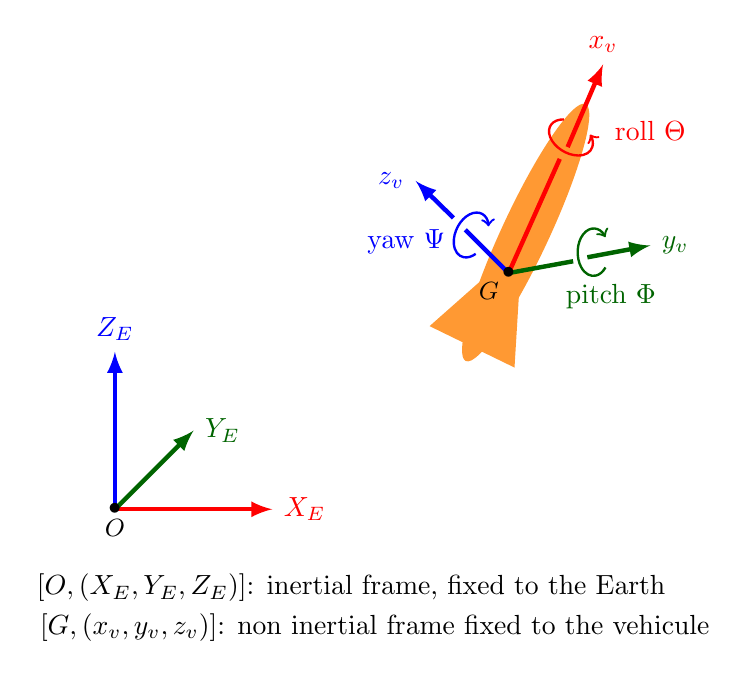
\begin{tikzpicture}
	\begin{pgfonlayer}{foreground}
	
	  \draw[->, ultra thick, red,  arrows={-latex}]  (0,0) -- (2,0) node[right] {$X_E$};
	  \draw[->, ultra thick, DarkGreen,  arrows={-latex}]  (0,0) -- (1, 1) node[right] {$Y_E$};
	  \draw[->, ultra thick, blue,  arrows={-latex}]  (0,0) -- (0,2) node[above] {$Z_E$};
	  \draw  (0,0) node {\small $\bullet$};
	  \draw  (0,0) node[below] {\small $O$};
	
	  \draw[-, ultra thick, red] (5,3) -- (5.65, 4.45);
	  \draw[->, ultra thick, red,  arrows={-latex}]   (5.75,4.6) -- (6.2, 5.65) node[above] {$x_v$};
	  \draw[-, ultra thick, DarkGreen] (5,3) -- (5.82, 3.15);
	  \draw[->, ultra thick, DarkGreen, arrows={-latex}] (6.0,3.2) -- (6.8,3.35) node[right] {$y_v$};
	  \draw[-, ultra thick, blue]  (5,3) -- (4.45, 3.55);
	  \draw[->, ultra thick, blue,  arrows={-latex}]  (4.3, 3.7) -- (3.82, 4.17) node[left] {$z_v$};
	  \draw  (5,3) node {\small $\bullet$};
	  \draw  (5,3) node[below left] {\small $G$};
 
	  \end{pgfonlayer}
 
 
	  \draw[] node[isosceles triangle, fill=orange!80, minimum size=12mm, rotate=64] (T) at (4.7,2.4){};
	  \fill[orange!80, rotate=-25, yshift=68, xshift=-50] (5,3) ellipse(0.3 and 1.8);
 
	  \draw[line width=.3mm,color=red, ->, yshift=-25, xshift=165, rotate=60] 
	  (5,3) arc (40:320:2mm and 3mm);
	  \draw[red] (6.8, 4.8) node{roll $\Theta$};
 
	  \draw[line width=.3mm,color=DarkGreen, <-, yshift=13, xshift=35, rotate=0] 
	  (5,3) arc (40:320:2mm and 3mm);
	  \draw[DarkGreen]  (6.3, 2.7) node{pitch $\Phi$};
	  
	  \draw[line width=.3mm,color=blue, <-, yshift=85, xshift=-30, rotate=-25] 
	  (5,3) arc (40:320:2mm and 3mm);
	  \draw[blue]  (3.7, 3.4) node{yaw $\Psi$};
	  
	  \draw (3, -1) node {$[O, (\vect{X_E},\vect{Y_E}, \vect{Z_E})]$: inertial frame, fixed to the Earth};
	  \draw (3.3, -1.5) node {$[G, (\vect{x_v},\vect{y_v},\vect{z_v})]$: non inertial frame fixed to the vehicule};

\end{tikzpicture}

\end{document}    
